\documentclass[twoside]{book}

% Packages required by doxygen
\usepackage{calc}
\usepackage{doxygen}
\usepackage{graphicx}
\usepackage[utf8]{inputenc}
\usepackage{makeidx}
\usepackage{multicol}
\usepackage{multirow}
\usepackage{textcomp}
\usepackage[table]{xcolor}

% Font selection
\usepackage[T1]{fontenc}
\usepackage{mathptmx}
\usepackage[scaled=.90]{helvet}
\usepackage{courier}
\usepackage{amssymb}
\usepackage{sectsty}
\renewcommand{\familydefault}{\sfdefault}
\allsectionsfont{%
  \fontseries{bc}\selectfont%
  \color{darkgray}%
}
\renewcommand{\DoxyLabelFont}{%
  \fontseries{bc}\selectfont%
  \color{darkgray}%
}

% Page & text layout
\usepackage{geometry}
\geometry{%
  a4paper,%
  top=2.5cm,%
  bottom=2.5cm,%
  left=2.5cm,%
  right=2.5cm%
}
\tolerance=750
\hfuzz=15pt
\hbadness=750
\setlength{\emergencystretch}{15pt}
\setlength{\parindent}{0cm}
\setlength{\parskip}{0.2cm}
\makeatletter
\renewcommand{\paragraph}{%
  \@startsection{paragraph}{4}{0ex}{-1.0ex}{1.0ex}{%
    \normalfont\normalsize\bfseries\SS@parafont%
  }%
}
\renewcommand{\subparagraph}{%
  \@startsection{subparagraph}{5}{0ex}{-1.0ex}{1.0ex}{%
    \normalfont\normalsize\bfseries\SS@subparafont%
  }%
}
\makeatother

% Headers & footers
\usepackage{fancyhdr}
\pagestyle{fancyplain}
\fancyhead[LE]{\fancyplain{}{\bfseries\thepage}}
\fancyhead[CE]{\fancyplain{}{}}
\fancyhead[RE]{\fancyplain{}{\bfseries\leftmark}}
\fancyhead[LO]{\fancyplain{}{\bfseries\rightmark}}
\fancyhead[CO]{\fancyplain{}{}}
\fancyhead[RO]{\fancyplain{}{\bfseries\thepage}}
\fancyfoot[LE]{\fancyplain{}{}}
\fancyfoot[CE]{\fancyplain{}{}}
\fancyfoot[RE]{\fancyplain{}{\bfseries\scriptsize Generated on Mon Mar 28 2016 00\-:15\-:01 for My Project by Doxygen }}
\fancyfoot[LO]{\fancyplain{}{\bfseries\scriptsize Generated on Mon Mar 28 2016 00\-:15\-:01 for My Project by Doxygen }}
\fancyfoot[CO]{\fancyplain{}{}}
\fancyfoot[RO]{\fancyplain{}{}}
\renewcommand{\footrulewidth}{0.4pt}
\renewcommand{\chaptermark}[1]{%
  \markboth{#1}{}%
}
\renewcommand{\sectionmark}[1]{%
  \markright{\thesection\ #1}%
}

% Indices & bibliography
\usepackage{natbib}
\usepackage[titles]{tocloft}
\setcounter{tocdepth}{3}
\setcounter{secnumdepth}{5}
\makeindex

% Hyperlinks (required, but should be loaded last)
\usepackage{ifpdf}
\ifpdf
  \usepackage[pdftex,pagebackref=true]{hyperref}
\else
  \usepackage[ps2pdf,pagebackref=true]{hyperref}
\fi
\hypersetup{%
  colorlinks=true,%
  linkcolor=blue,%
  citecolor=blue,%
  unicode%
}

% Custom commands
\newcommand{\clearemptydoublepage}{%
  \newpage{\pagestyle{empty}\cleardoublepage}%
}


%===== C O N T E N T S =====

\begin{document}

% Titlepage & ToC
\hypersetup{pageanchor=false}
\pagenumbering{roman}
\begin{titlepage}
\vspace*{7cm}
\begin{center}%
{\Large My Project }\\
\vspace*{1cm}
{\large Generated by Doxygen 1.8.6}\\
\vspace*{0.5cm}
{\small Mon Mar 28 2016 00:15:01}\\
\end{center}
\end{titlepage}
\clearemptydoublepage
\tableofcontents
\clearemptydoublepage
\pagenumbering{arabic}
\hypersetup{pageanchor=true}

%--- Begin generated contents ---
\chapter{Hierarchical Index}
\section{Class Hierarchy}
This inheritance list is sorted roughly, but not completely, alphabetically\-:\begin{DoxyCompactList}
\item \contentsline{section}{Dictionary}{\pageref{class_dictionary}}{}
\begin{DoxyCompactList}
\item \contentsline{section}{Lista}{\pageref{class_lista}}{}
\begin{DoxyCompactList}
\item \contentsline{section}{Lista\-Test}{\pageref{class_lista_test}}{}
\end{DoxyCompactList}
\end{DoxyCompactList}
\item \contentsline{section}{I\-List}{\pageref{class_i_list}}{}
\begin{DoxyCompactList}
\item \contentsline{section}{Lista}{\pageref{class_lista}}{}
\end{DoxyCompactList}
\item \contentsline{section}{I\-Queue}{\pageref{class_i_queue}}{}
\begin{DoxyCompactList}
\item \contentsline{section}{Kolejka}{\pageref{class_kolejka}}{}
\begin{DoxyCompactList}
\item \contentsline{section}{Kolejka\-Test}{\pageref{class_kolejka_test}}{}
\item \contentsline{section}{Lista}{\pageref{class_lista}}{}
\end{DoxyCompactList}
\end{DoxyCompactList}
\item \contentsline{section}{I\-Runnable}{\pageref{class_i_runnable}}{}
\begin{DoxyCompactList}
\item \contentsline{section}{Kolejka\-Test}{\pageref{class_kolejka_test}}{}
\item \contentsline{section}{Lista\-Test}{\pageref{class_lista_test}}{}
\end{DoxyCompactList}
\item \contentsline{section}{I\-Stack}{\pageref{class_i_stack}}{}
\begin{DoxyCompactList}
\item \contentsline{section}{Stos}{\pageref{class_stos}}{}
\end{DoxyCompactList}
\item \contentsline{section}{Sorting\-Alg}{\pageref{class_sorting_alg}}{}
\item \contentsline{section}{Stopwatch}{\pageref{class_stopwatch}}{}
\begin{DoxyCompactList}
\item \contentsline{section}{Lista}{\pageref{class_lista}}{}
\end{DoxyCompactList}
\end{DoxyCompactList}

\chapter{Class Index}
\section{Class List}
Here are the classes, structs, unions and interfaces with brief descriptions\-:\begin{DoxyCompactList}
\item\contentsline{section}{\hyperlink{class_dictionary}{Dictionary} }{\pageref{class_dictionary}}{}
\item\contentsline{section}{\hyperlink{class_i_list}{I\-List} }{\pageref{class_i_list}}{}
\item\contentsline{section}{\hyperlink{class_i_queue}{I\-Queue} }{\pageref{class_i_queue}}{}
\item\contentsline{section}{\hyperlink{class_i_runnable}{I\-Runnable} }{\pageref{class_i_runnable}}{}
\item\contentsline{section}{\hyperlink{class_i_stack}{I\-Stack} }{\pageref{class_i_stack}}{}
\item\contentsline{section}{\hyperlink{class_kolejka}{Kolejka} }{\pageref{class_kolejka}}{}
\item\contentsline{section}{\hyperlink{class_kolejka_test}{Kolejka\-Test} }{\pageref{class_kolejka_test}}{}
\item\contentsline{section}{\hyperlink{class_lista}{Lista} }{\pageref{class_lista}}{}
\item\contentsline{section}{\hyperlink{class_lista_test}{Lista\-Test} }{\pageref{class_lista_test}}{}
\item\contentsline{section}{\hyperlink{class_sorting_alg}{Sorting\-Alg} }{\pageref{class_sorting_alg}}{}
\item\contentsline{section}{\hyperlink{class_stopwatch}{Stopwatch} }{\pageref{class_stopwatch}}{}
\item\contentsline{section}{\hyperlink{class_stos}{Stos} }{\pageref{class_stos}}{}
\end{DoxyCompactList}

\chapter{Class Documentation}
\hypertarget{class_dictionary}{\section{Dictionary Class Reference}
\label{class_dictionary}\index{Dictionary@{Dictionary}}
}
Inheritance diagram for Dictionary\-:\begin{figure}[H]
\begin{center}
\leavevmode
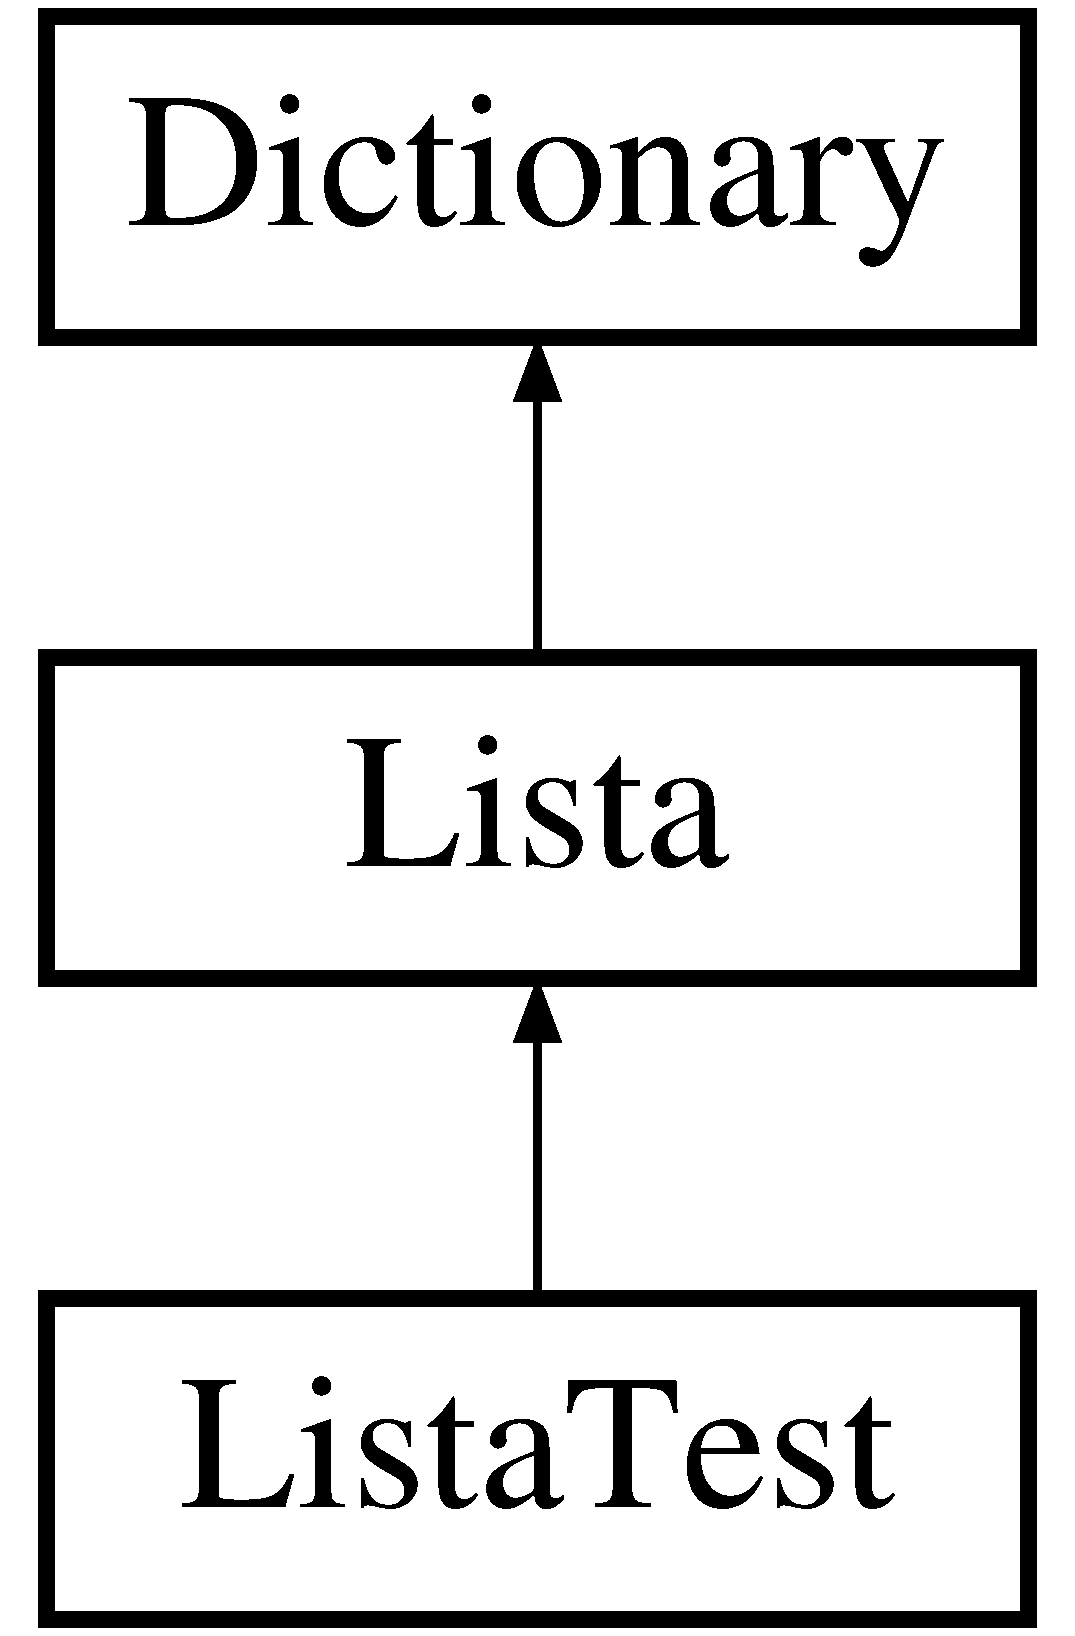
\includegraphics[height=3.000000cm]{class_dictionary}
\end{center}
\end{figure}
\subsection*{Public Member Functions}
\begin{DoxyCompactItemize}
\item 
void \hyperlink{class_dictionary_a5f7c40f501a0cf324dfea5a38d974eed}{set\-Words} ()
\item 
string \hyperlink{class_dictionary_a5bd0a1d493e52af07cf4bc3bbb1453d6}{get\-Words} (int i)
\item 
int \hyperlink{class_dictionary_a3466672e02319a215179f127fe0ae530}{count\-Lines} ()
\item 
string \hyperlink{class_dictionary_ad9c09209b38b2141be5438fd3ac14ebe}{Random\-Words} ()
\item 
int \hyperlink{class_dictionary_a267251a4e33289be24d0a945746aa54e}{Random\-Number} ()
\end{DoxyCompactItemize}


\subsection{Member Function Documentation}
\hypertarget{class_dictionary_a3466672e02319a215179f127fe0ae530}{\index{Dictionary@{Dictionary}!count\-Lines@{count\-Lines}}
\index{count\-Lines@{count\-Lines}!Dictionary@{Dictionary}}
\subsubsection[{count\-Lines}]{\setlength{\rightskip}{0pt plus 5cm}int Dictionary\-::count\-Lines (
\begin{DoxyParamCaption}
{}
\end{DoxyParamCaption}
)}}\label{class_dictionary_a3466672e02319a215179f127fe0ae530}
funkcja zliczajaca linie w pliku (ilosc slow w slowniku) \begin{DoxyReturn}{Returns}
lines 
\end{DoxyReturn}
\hypertarget{class_dictionary_a5bd0a1d493e52af07cf4bc3bbb1453d6}{\index{Dictionary@{Dictionary}!get\-Words@{get\-Words}}
\index{get\-Words@{get\-Words}!Dictionary@{Dictionary}}
\subsubsection[{get\-Words}]{\setlength{\rightskip}{0pt plus 5cm}string Dictionary\-::get\-Words (
\begin{DoxyParamCaption}
\item[{int}]{i}
\end{DoxyParamCaption}
)}}\label{class_dictionary_a5bd0a1d493e52af07cf4bc3bbb1453d6}
funkcja zwracajaca slowo z tablicy z wyrazami ze slownika 
\begin{DoxyParams}{Parameters}
{\em i} & -\/ numer indeksu zwracanego slowa \\
\hline
\end{DoxyParams}
\begin{DoxyReturn}{Returns}
words\-\_\-\mbox{[}i\mbox{]} 
\end{DoxyReturn}
\hypertarget{class_dictionary_a267251a4e33289be24d0a945746aa54e}{\index{Dictionary@{Dictionary}!Random\-Number@{Random\-Number}}
\index{Random\-Number@{Random\-Number}!Dictionary@{Dictionary}}
\subsubsection[{Random\-Number}]{\setlength{\rightskip}{0pt plus 5cm}int Dictionary\-::\-Random\-Number (
\begin{DoxyParamCaption}
{}
\end{DoxyParamCaption}
)}}\label{class_dictionary_a267251a4e33289be24d0a945746aa54e}
funkcja generujaca losowe liczby \begin{DoxyReturn}{Returns}

\end{DoxyReturn}
\hypertarget{class_dictionary_ad9c09209b38b2141be5438fd3ac14ebe}{\index{Dictionary@{Dictionary}!Random\-Words@{Random\-Words}}
\index{Random\-Words@{Random\-Words}!Dictionary@{Dictionary}}
\subsubsection[{Random\-Words}]{\setlength{\rightskip}{0pt plus 5cm}string Dictionary\-::\-Random\-Words (
\begin{DoxyParamCaption}
{}
\end{DoxyParamCaption}
)}}\label{class_dictionary_ad9c09209b38b2141be5438fd3ac14ebe}
funkcja generujaca losowe slowa na podstawie slownika \begin{DoxyReturn}{Returns}

\end{DoxyReturn}
\hypertarget{class_dictionary_a5f7c40f501a0cf324dfea5a38d974eed}{\index{Dictionary@{Dictionary}!set\-Words@{set\-Words}}
\index{set\-Words@{set\-Words}!Dictionary@{Dictionary}}
\subsubsection[{set\-Words}]{\setlength{\rightskip}{0pt plus 5cm}void Dictionary\-::set\-Words (
\begin{DoxyParamCaption}
{}
\end{DoxyParamCaption}
)}}\label{class_dictionary_a5f7c40f501a0cf324dfea5a38d974eed}
funkcja wczytujaca slownik do tablicy 

The documentation for this class was generated from the following files\-:\begin{DoxyCompactItemize}
\item 
Dictionary.\-h\item 
Dictionary.\-cpp\end{DoxyCompactItemize}

\hypertarget{class_i_list}{\section{I\-List Class Reference}
\label{class_i_list}\index{I\-List@{I\-List}}
}
Inheritance diagram for I\-List\-:\begin{figure}[H]
\begin{center}
\leavevmode
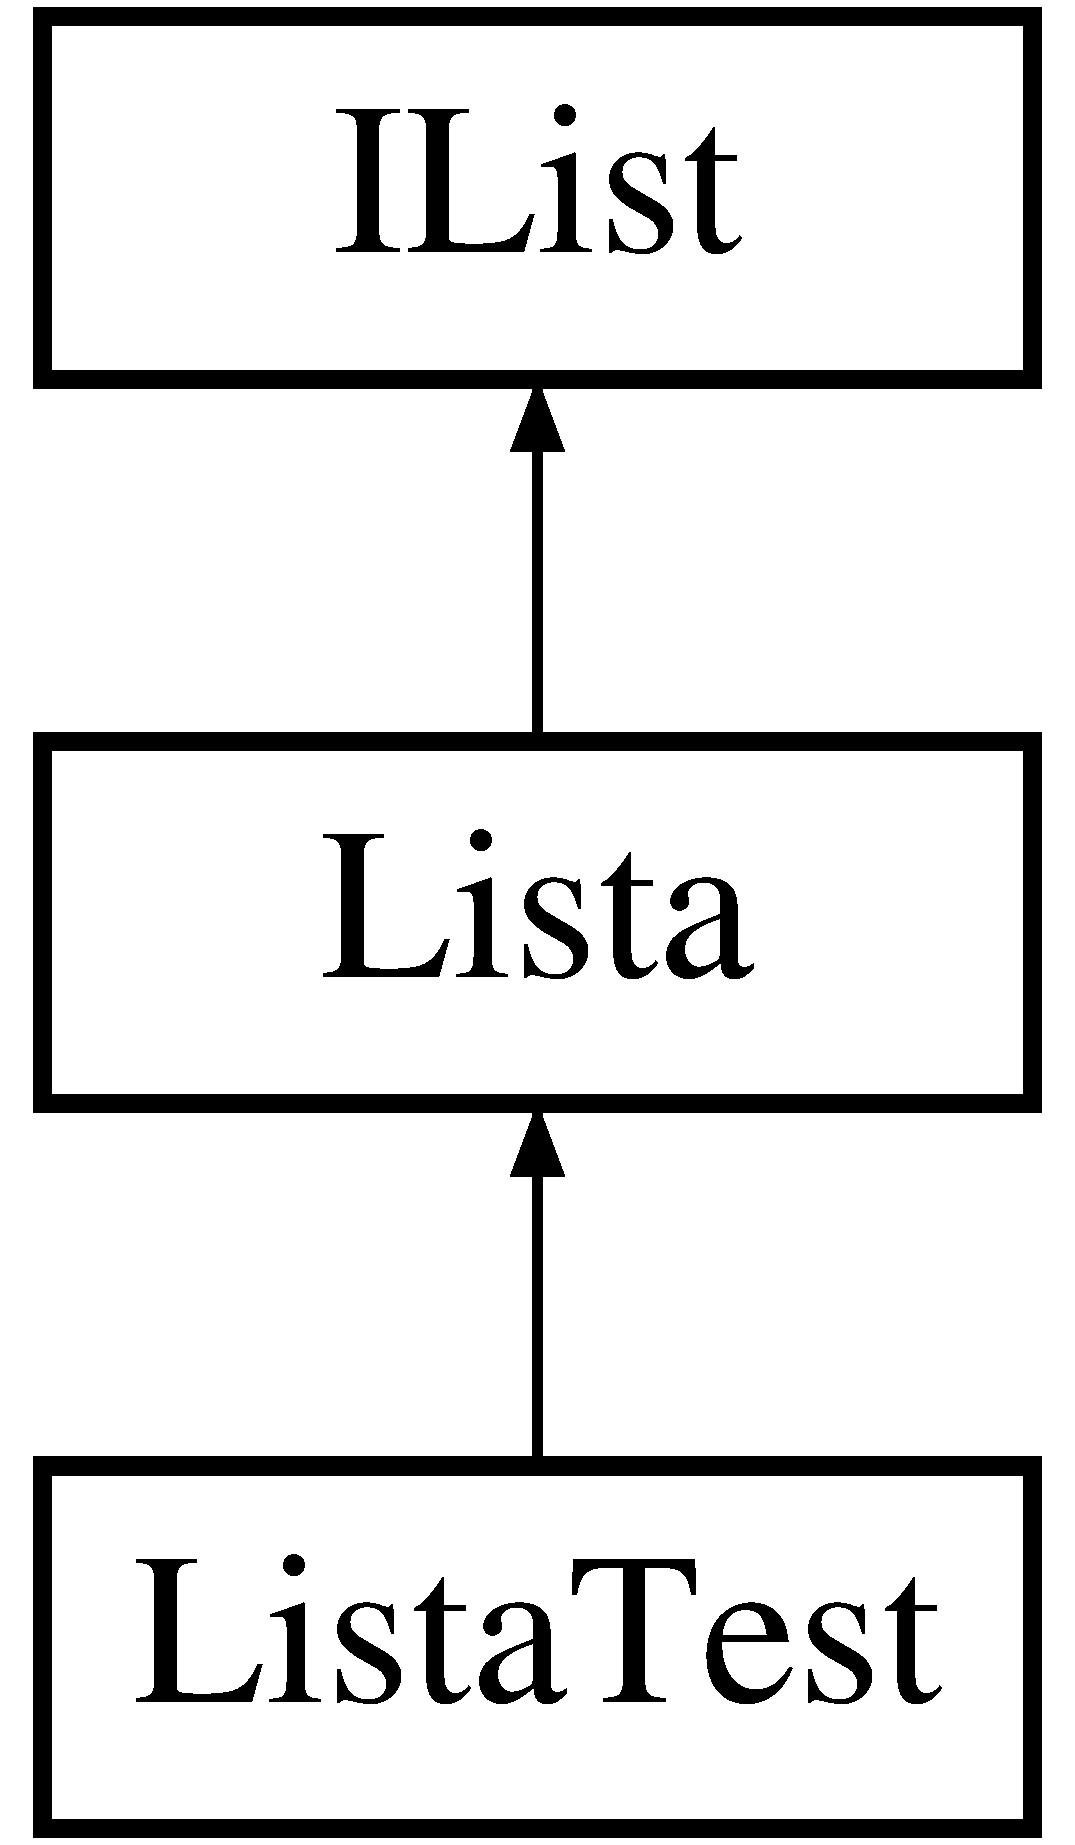
\includegraphics[height=3.000000cm]{class_i_list}
\end{center}
\end{figure}
\subsection*{Public Member Functions}
\begin{DoxyCompactItemize}
\item 
\hypertarget{class_i_list_ab79348ba7116b9a204b2f7f389e2f3e9}{int {\bfseries size} ()}\label{class_i_list_ab79348ba7116b9a204b2f7f389e2f3e9}

\item 
\hypertarget{class_i_list_a1ab72644b90e917b927de7392aea6af9}{void {\bfseries add} (int a)}\label{class_i_list_a1ab72644b90e917b927de7392aea6af9}

\item 
\hypertarget{class_i_list_a7db3e8a2b0dfc7bd3c1fcecea79f2f1b}{void {\bfseries remove} ()}\label{class_i_list_a7db3e8a2b0dfc7bd3c1fcecea79f2f1b}

\item 
\hypertarget{class_i_list_a6c7987cdd1aeb40da2df1ae9e91d59c4}{int {\bfseries get\-Elem} (int index)}\label{class_i_list_a6c7987cdd1aeb40da2df1ae9e91d59c4}

\end{DoxyCompactItemize}


The documentation for this class was generated from the following files\-:\begin{DoxyCompactItemize}
\item 
I\-List.\-h\item 
I\-List.\-cpp\end{DoxyCompactItemize}

\hypertarget{class_i_queue}{\section{I\-Queue Class Reference}
\label{class_i_queue}\index{I\-Queue@{I\-Queue}}
}
Inheritance diagram for I\-Queue\-:\begin{figure}[H]
\begin{center}
\leavevmode
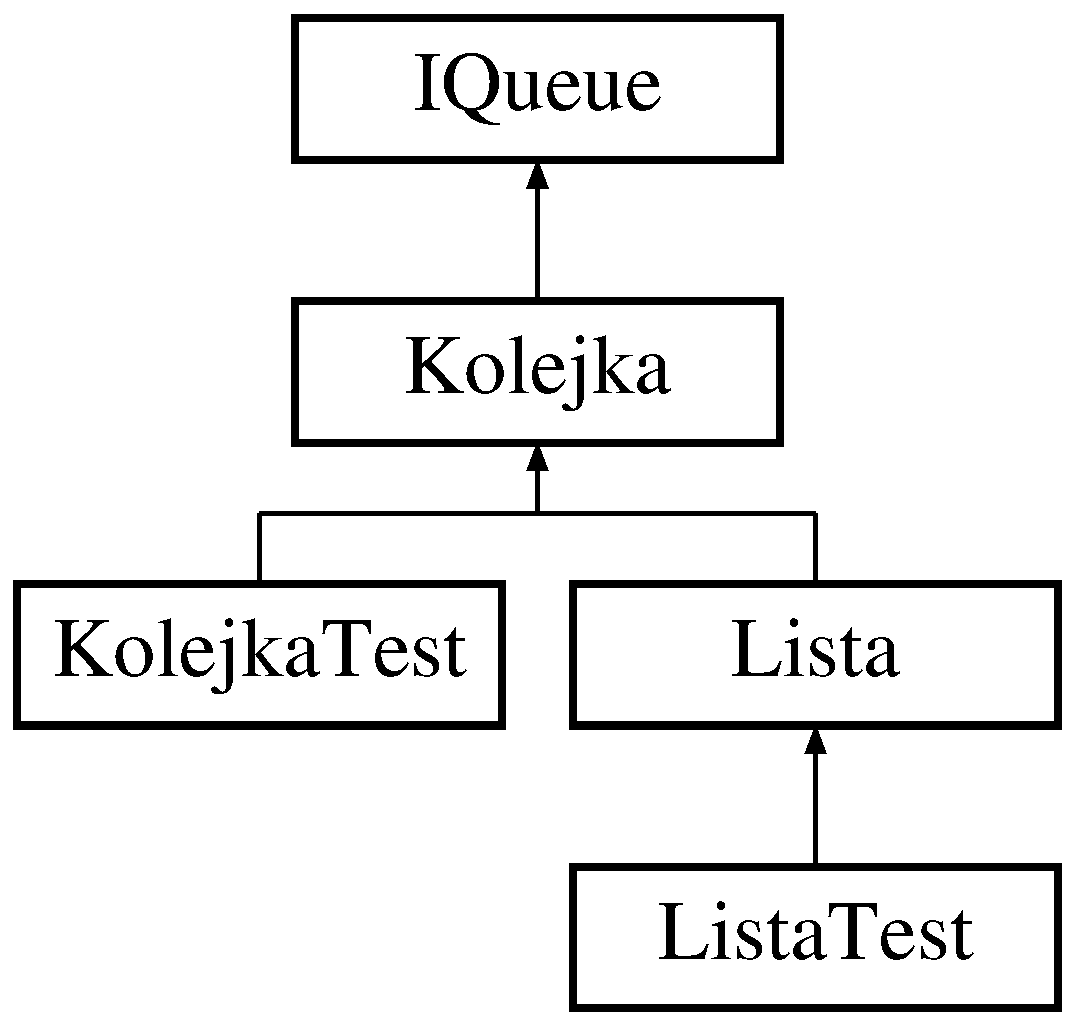
\includegraphics[height=4.000000cm]{class_i_queue}
\end{center}
\end{figure}
\subsection*{Public Member Functions}
\begin{DoxyCompactItemize}
\item 
\hypertarget{class_i_queue_ac751567102d944b59366acaece0ca639}{virtual void {\bfseries enqueue} (int a)=0}\label{class_i_queue_ac751567102d944b59366acaece0ca639}

\item 
\hypertarget{class_i_queue_a99998d398d9e13ebbf47596c1d9cc9f3}{int {\bfseries size} ()}\label{class_i_queue_a99998d398d9e13ebbf47596c1d9cc9f3}

\item 
\hypertarget{class_i_queue_a243ebb1847cb1210d8d7e32b6b602bdb}{bool {\bfseries is\-Empty} ()}\label{class_i_queue_a243ebb1847cb1210d8d7e32b6b602bdb}

\item 
\hypertarget{class_i_queue_a3d2dbf94af124d9c74e88f862b25ee31}{void {\bfseries dequeue} ()}\label{class_i_queue_a3d2dbf94af124d9c74e88f862b25ee31}

\end{DoxyCompactItemize}


The documentation for this class was generated from the following files\-:\begin{DoxyCompactItemize}
\item 
I\-Queue.\-h\item 
I\-Queue.\-cpp\end{DoxyCompactItemize}

\hypertarget{class_i_runnable}{\section{I\-Runnable Class Reference}
\label{class_i_runnable}\index{I\-Runnable@{I\-Runnable}}
}
Inheritance diagram for I\-Runnable\-:\begin{figure}[H]
\begin{center}
\leavevmode
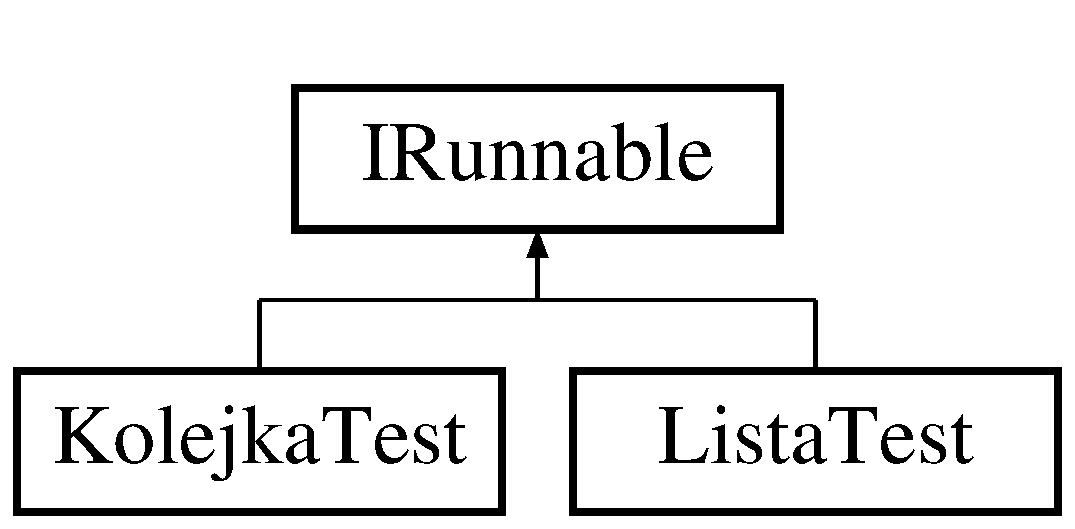
\includegraphics[height=2.000000cm]{class_i_runnable}
\end{center}
\end{figure}
\subsection*{Public Member Functions}
\begin{DoxyCompactItemize}
\item 
\hypertarget{class_i_runnable_ad830df095945f75563d27c2ee8bae0f5}{virtual void {\bfseries run} (int Amount\-Of\-Comp)=0}\label{class_i_runnable_ad830df095945f75563d27c2ee8bae0f5}

\end{DoxyCompactItemize}


The documentation for this class was generated from the following files\-:\begin{DoxyCompactItemize}
\item 
I\-Runnable.\-h\item 
I\-Runnable.\-cpp\end{DoxyCompactItemize}

\hypertarget{class_i_stack}{\section{I\-Stack Class Reference}
\label{class_i_stack}\index{I\-Stack@{I\-Stack}}
}
Inheritance diagram for I\-Stack\-:\begin{figure}[H]
\begin{center}
\leavevmode
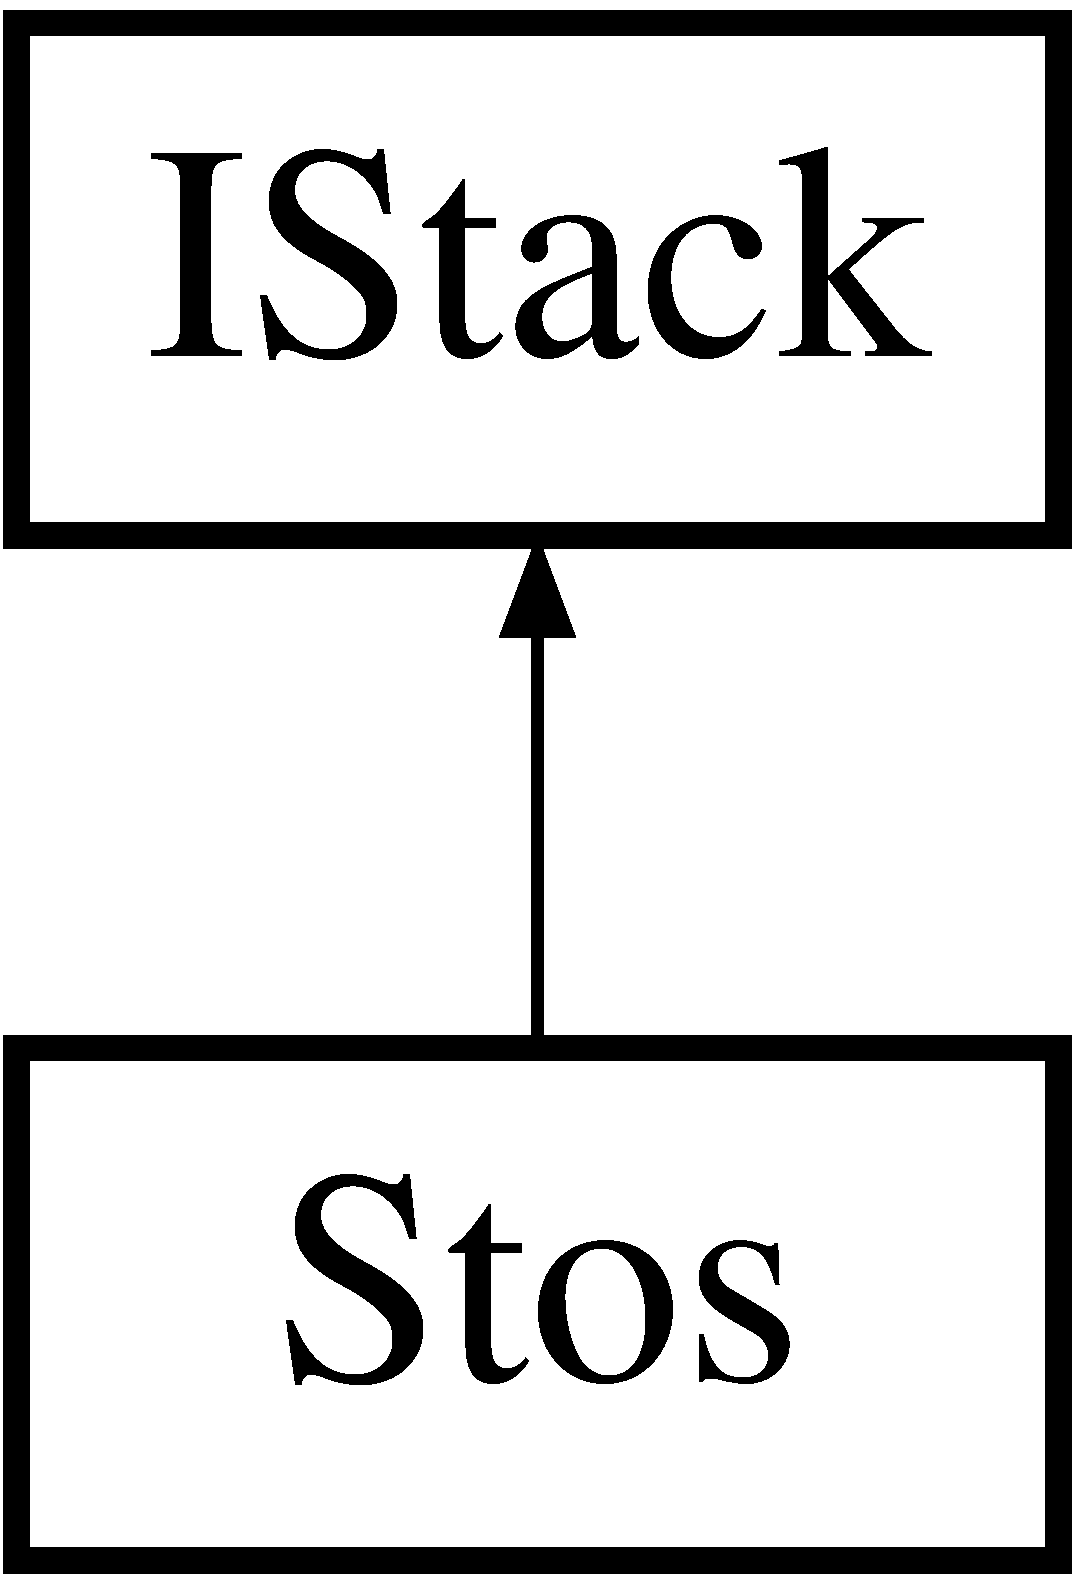
\includegraphics[height=2.000000cm]{class_i_stack}
\end{center}
\end{figure}
\subsection*{Public Member Functions}
\begin{DoxyCompactItemize}
\item 
\hypertarget{class_i_stack_aaea872f831c1ab5c064bed14f552e1fe}{int {\bfseries get\-Size} ()}\label{class_i_stack_aaea872f831c1ab5c064bed14f552e1fe}

\item 
\hypertarget{class_i_stack_a237e08de5a3cebe1266c5f4e038fa2e3}{bool {\bfseries is\-Empty} ()}\label{class_i_stack_a237e08de5a3cebe1266c5f4e038fa2e3}

\item 
\hypertarget{class_i_stack_ab2daefea39cc1ff2c2e1889a0acc6373}{int {\bfseries top} ()}\label{class_i_stack_ab2daefea39cc1ff2c2e1889a0acc6373}

\item 
\hypertarget{class_i_stack_a6f1563e90b6e1194c0e8415fa0275138}{void {\bfseries push} (int a)}\label{class_i_stack_a6f1563e90b6e1194c0e8415fa0275138}

\item 
\hypertarget{class_i_stack_a9bcbe8c107e81e4d92f8707382d0a6d1}{int {\bfseries pop} ()}\label{class_i_stack_a9bcbe8c107e81e4d92f8707382d0a6d1}

\end{DoxyCompactItemize}


The documentation for this class was generated from the following files\-:\begin{DoxyCompactItemize}
\item 
I\-Stack.\-h\item 
I\-Stack.\-cpp\end{DoxyCompactItemize}

\hypertarget{class_kolejka}{\section{Kolejka Class Reference}
\label{class_kolejka}\index{Kolejka@{Kolejka}}
}
Inheritance diagram for Kolejka\-:\begin{figure}[H]
\begin{center}
\leavevmode
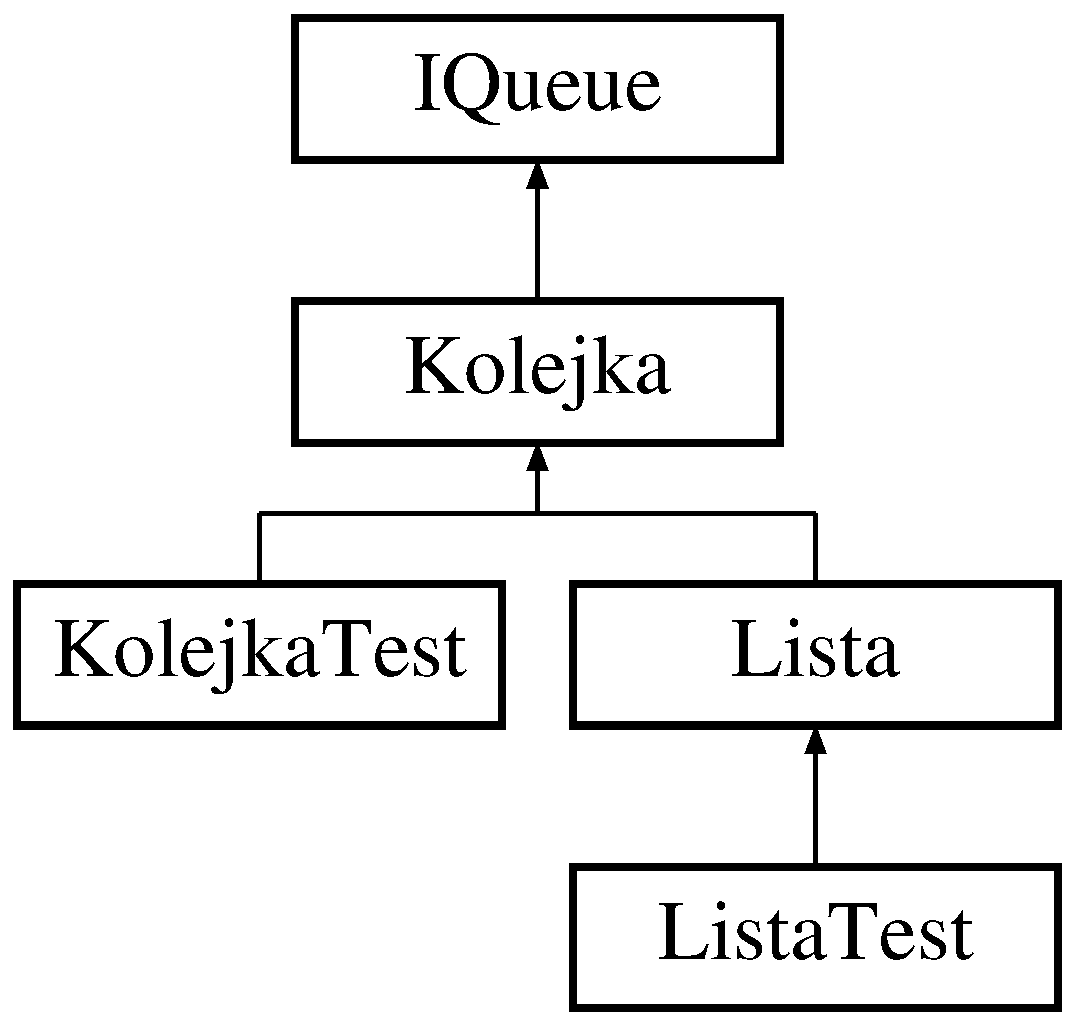
\includegraphics[height=4.000000cm]{class_kolejka}
\end{center}
\end{figure}
\subsection*{Public Member Functions}
\begin{DoxyCompactItemize}
\item 
\hyperlink{class_kolejka_a37c886fdc73dce62b04da0381dec5484}{Kolejka} ()
\item 
int \hyperlink{class_kolejka_a0cce8b13fa5328bcbad40eec7906fd37}{get\-Size} ()
\item 
void \hyperlink{class_kolejka_abe885467bd893eef589edc8da595933c}{enqueue} (int a)
\item 
void \hyperlink{class_kolejka_a7ab02bd0f86d6994b6aeb344bc1d025e}{display} ()
\item 
void \hyperlink{class_kolejka_a9c78c81b3ef4d4d7a54215ab7fe380ff}{dequeue} ()
\item 
bool \hyperlink{class_kolejka_a0106bd9157a970b63a06edd1dad350a9}{is\-Empty} ()
\item 
int \hyperlink{class_kolejka_a814f1ec21256de252aa6f74bf78bf69e}{get\-Front} ()
\item 
int \hyperlink{class_kolejka_a8a0847d6da0a51f79d7d6baa271ca261}{get\-Rear} ()
\end{DoxyCompactItemize}


\subsection{Constructor \& Destructor Documentation}
\hypertarget{class_kolejka_a37c886fdc73dce62b04da0381dec5484}{\index{Kolejka@{Kolejka}!Kolejka@{Kolejka}}
\index{Kolejka@{Kolejka}!Kolejka@{Kolejka}}
\subsubsection[{Kolejka}]{\setlength{\rightskip}{0pt plus 5cm}Kolejka\-::\-Kolejka (
\begin{DoxyParamCaption}
{}
\end{DoxyParamCaption}
)}}\label{class_kolejka_a37c886fdc73dce62b04da0381dec5484}
konstruktor size\-\_\--\/poczatkowy rozmiar kolejki front\-\_\- -\/ pierwszy element w kolejce rear\-\_\- -\/ ostatni element w kolejce count\-\_\- -\/ licznik elementow w kolejce 

\subsection{Member Function Documentation}
\hypertarget{class_kolejka_a9c78c81b3ef4d4d7a54215ab7fe380ff}{\index{Kolejka@{Kolejka}!dequeue@{dequeue}}
\index{dequeue@{dequeue}!Kolejka@{Kolejka}}
\subsubsection[{dequeue}]{\setlength{\rightskip}{0pt plus 5cm}void Kolejka\-::dequeue (
\begin{DoxyParamCaption}
{}
\end{DoxyParamCaption}
)}}\label{class_kolejka_a9c78c81b3ef4d4d7a54215ab7fe380ff}
funkcja usuwajaca element z poczatku kolejki \hypertarget{class_kolejka_a7ab02bd0f86d6994b6aeb344bc1d025e}{\index{Kolejka@{Kolejka}!display@{display}}
\index{display@{display}!Kolejka@{Kolejka}}
\subsubsection[{display}]{\setlength{\rightskip}{0pt plus 5cm}void Kolejka\-::display (
\begin{DoxyParamCaption}
{}
\end{DoxyParamCaption}
)}}\label{class_kolejka_a7ab02bd0f86d6994b6aeb344bc1d025e}
funkcja wyswietlajaca kolejke \hypertarget{class_kolejka_abe885467bd893eef589edc8da595933c}{\index{Kolejka@{Kolejka}!enqueue@{enqueue}}
\index{enqueue@{enqueue}!Kolejka@{Kolejka}}
\subsubsection[{enqueue}]{\setlength{\rightskip}{0pt plus 5cm}void Kolejka\-::enqueue (
\begin{DoxyParamCaption}
\item[{int}]{a}
\end{DoxyParamCaption}
)\hspace{0.3cm}{\ttfamily [virtual]}}}\label{class_kolejka_abe885467bd893eef589edc8da595933c}
funkcja dodajaca element na koncu kolejki 

Implements \hyperlink{class_i_queue}{I\-Queue}.

\hypertarget{class_kolejka_a814f1ec21256de252aa6f74bf78bf69e}{\index{Kolejka@{Kolejka}!get\-Front@{get\-Front}}
\index{get\-Front@{get\-Front}!Kolejka@{Kolejka}}
\subsubsection[{get\-Front}]{\setlength{\rightskip}{0pt plus 5cm}int Kolejka\-::get\-Front (
\begin{DoxyParamCaption}
{}
\end{DoxyParamCaption}
)}}\label{class_kolejka_a814f1ec21256de252aa6f74bf78bf69e}
funkcja zwracajaca wartosc pierwszego elementu w kolejce \begin{DoxyReturn}{Returns}

\end{DoxyReturn}
\hypertarget{class_kolejka_a8a0847d6da0a51f79d7d6baa271ca261}{\index{Kolejka@{Kolejka}!get\-Rear@{get\-Rear}}
\index{get\-Rear@{get\-Rear}!Kolejka@{Kolejka}}
\subsubsection[{get\-Rear}]{\setlength{\rightskip}{0pt plus 5cm}int Kolejka\-::get\-Rear (
\begin{DoxyParamCaption}
{}
\end{DoxyParamCaption}
)}}\label{class_kolejka_a8a0847d6da0a51f79d7d6baa271ca261}
funkcja zwracajaca wartosc ostatneig elementu w kolejce \begin{DoxyReturn}{Returns}

\end{DoxyReturn}
\hypertarget{class_kolejka_a0cce8b13fa5328bcbad40eec7906fd37}{\index{Kolejka@{Kolejka}!get\-Size@{get\-Size}}
\index{get\-Size@{get\-Size}!Kolejka@{Kolejka}}
\subsubsection[{get\-Size}]{\setlength{\rightskip}{0pt plus 5cm}int Kolejka\-::get\-Size (
\begin{DoxyParamCaption}
{}
\end{DoxyParamCaption}
)}}\label{class_kolejka_a0cce8b13fa5328bcbad40eec7906fd37}
funkcja, ktora zwraca rozmiar kolejki \begin{DoxyReturn}{Returns}

\end{DoxyReturn}
\hypertarget{class_kolejka_a0106bd9157a970b63a06edd1dad350a9}{\index{Kolejka@{Kolejka}!is\-Empty@{is\-Empty}}
\index{is\-Empty@{is\-Empty}!Kolejka@{Kolejka}}
\subsubsection[{is\-Empty}]{\setlength{\rightskip}{0pt plus 5cm}bool Kolejka\-::is\-Empty (
\begin{DoxyParamCaption}
{}
\end{DoxyParamCaption}
)}}\label{class_kolejka_a0106bd9157a970b63a06edd1dad350a9}
funkcja, ktora sprawdza, czy kolejka jest pusta, zwraca 1, gdy tak \begin{DoxyReturn}{Returns}

\end{DoxyReturn}


The documentation for this class was generated from the following files\-:\begin{DoxyCompactItemize}
\item 
Kolejka.\-h\item 
Kolejka.\-cpp\end{DoxyCompactItemize}

\hypertarget{class_kolejka_test}{\section{Kolejka\-Test Class Reference}
\label{class_kolejka_test}\index{Kolejka\-Test@{Kolejka\-Test}}
}
Inheritance diagram for Kolejka\-Test\-:\begin{figure}[H]
\begin{center}
\leavevmode
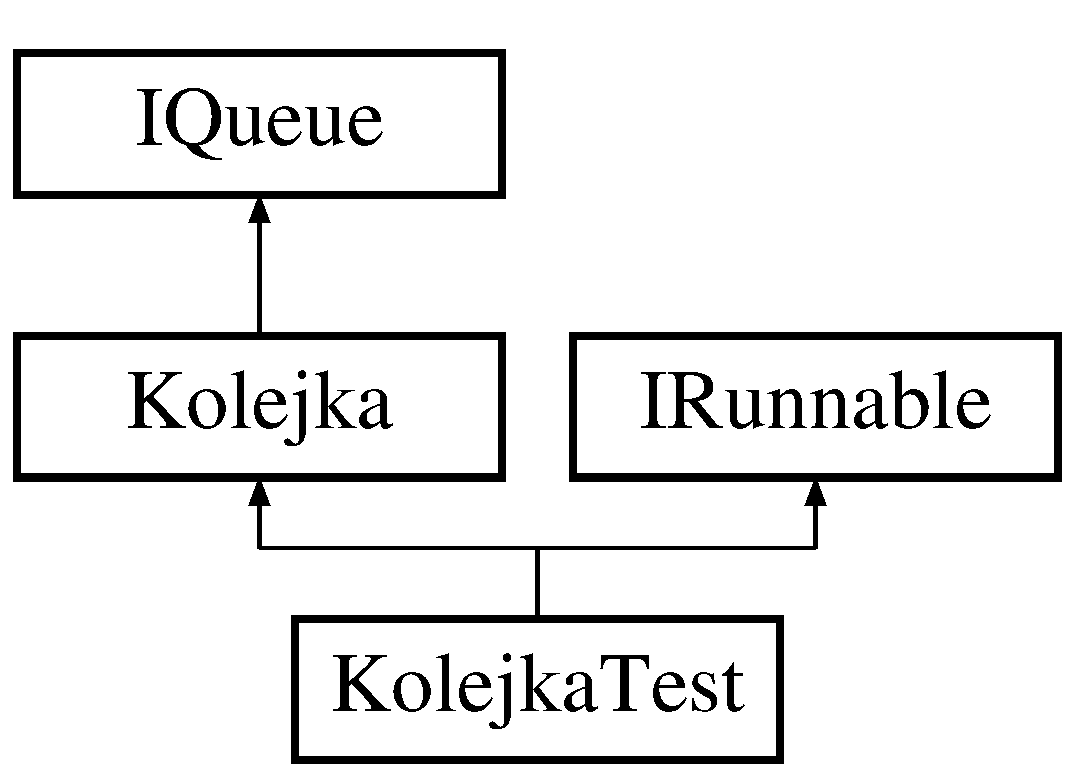
\includegraphics[height=3.000000cm]{class_kolejka_test}
\end{center}
\end{figure}
\subsection*{Public Member Functions}
\begin{DoxyCompactItemize}
\item 
\hypertarget{class_kolejka_test_a3a0bf78ef7f07ce376a60e7a205f7b45}{void {\bfseries run} (int Amount\-Of\-Comp)}\label{class_kolejka_test_a3a0bf78ef7f07ce376a60e7a205f7b45}

\end{DoxyCompactItemize}


The documentation for this class was generated from the following files\-:\begin{DoxyCompactItemize}
\item 
Kolejka\-Test.\-h\item 
Kolejka\-Test.\-cpp\end{DoxyCompactItemize}

\hypertarget{class_lista}{\section{Lista Class Reference}
\label{class_lista}\index{Lista@{Lista}}
}
Inheritance diagram for Lista\-:\begin{figure}[H]
\begin{center}
\leavevmode
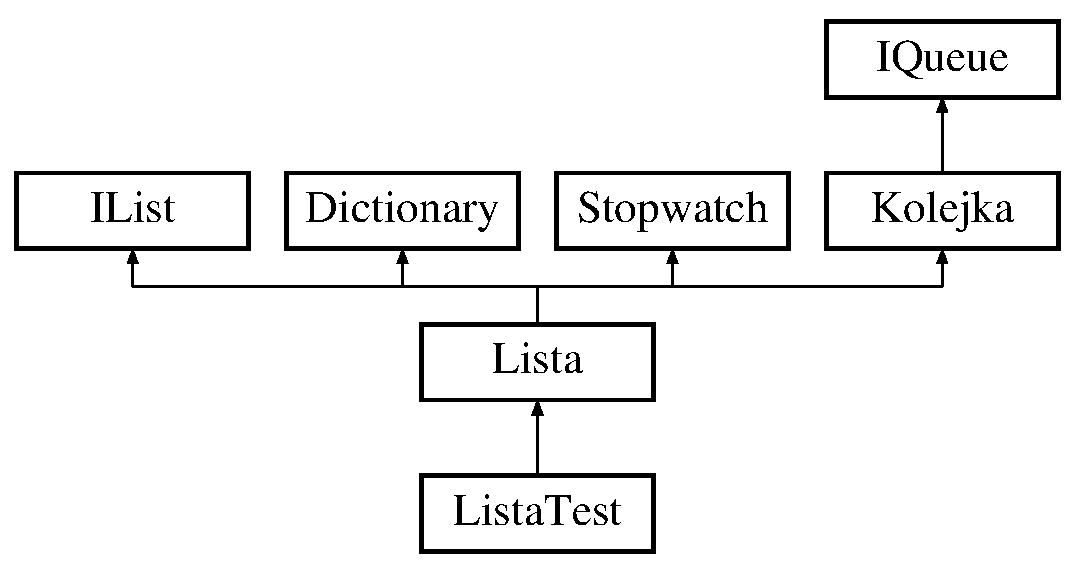
\includegraphics[height=4.000000cm]{class_lista}
\end{center}
\end{figure}
\subsection*{Public Member Functions}
\begin{DoxyCompactItemize}
\item 
\hyperlink{class_lista_a1f668b36909182ef1360b48503529a31}{Lista} ()
\item 
virtual \hyperlink{class_lista_a4d7394b2728a00ad8404965b2e15d096}{$\sim$\-Lista} ()
\item 
void \hyperlink{class_lista_a537b5b7bdf21c955ced1da3805bf358a}{add} (string item, int position)
\begin{DoxyCompactList}\small\item\em position -\/ indeks elementu po ktorym mamy wstawic \end{DoxyCompactList}\item 
\hypertarget{class_lista_ac7c04bb24ccf464d2fef9d81fd9a02dd}{int {\bfseries get\-Elem} (int index)}\label{class_lista_ac7c04bb24ccf464d2fef9d81fd9a02dd}

\item 
int \hyperlink{class_lista_a8aa86fb2487cf9cb9167da8853ca3302}{get\-Size} ()
\item 
void \hyperlink{class_lista_a5ef1a17973150accfd4a090ef3523552}{display} (int i)
\begin{DoxyCompactList}\small\item\em wyswietla nazwe obiektu i numer indeksu obiektu, na ktory pokazuje jako nastepny \end{DoxyCompactList}\item 
int \hyperlink{class_lista_a292906bc7cfcf660965e4473031eab58}{find} (string item)
\item 
int \hyperlink{class_lista_af60ba64ffa74c296db48be95d3c3e631}{get\-Next} (int index)
\item 
string \hyperlink{class_lista_a6982ae8c93f39ceeec64a28eabf1f941}{get\-Name} (int index)
\item 
\hypertarget{class_lista_ac32257be6a2943e935709d1503b7214a}{bool {\bfseries is\-Empty} ()}\label{class_lista_ac32257be6a2943e935709d1503b7214a}

\item 
void \hyperlink{class_lista_a58de0d55144cbe5ef946068724ee3e2a}{remove} (int index)
\item 
int \hyperlink{class_lista_af69b912fbb339fb976c1d02c1ec2a5ed}{get\-Count} ()
\item 
\hypertarget{class_lista_a687d55dc856ba92c3ece5be4c241f36f}{void {\bfseries display\-Free} ()}\label{class_lista_a687d55dc856ba92c3ece5be4c241f36f}

\end{DoxyCompactItemize}


\subsection{Constructor \& Destructor Documentation}
\hypertarget{class_lista_a1f668b36909182ef1360b48503529a31}{\index{Lista@{Lista}!Lista@{Lista}}
\index{Lista@{Lista}!Lista@{Lista}}
\subsubsection[{Lista}]{\setlength{\rightskip}{0pt plus 5cm}Lista\-::\-Lista (
\begin{DoxyParamCaption}
{}
\end{DoxyParamCaption}
)}}\label{class_lista_a1f668b36909182ef1360b48503529a31}
konstruktorsize\-\_\-=S\-I\-Z\-E -\/ poczatkowy rozmiar listy count\-\_\- -\/ liczba elementow na liscie end\-\_\-=0; name\-\_\- = -\/ tablica przechowujaca dodane elementy next\-\_\-= -\/ tablica przechowujaca indeks nastepnego elementu na liscie \hypertarget{class_lista_a4d7394b2728a00ad8404965b2e15d096}{\index{Lista@{Lista}!$\sim$\-Lista@{$\sim$\-Lista}}
\index{$\sim$\-Lista@{$\sim$\-Lista}!Lista@{Lista}}
\subsubsection[{$\sim$\-Lista}]{\setlength{\rightskip}{0pt plus 5cm}Lista\-::$\sim$\-Lista (
\begin{DoxyParamCaption}
{}
\end{DoxyParamCaption}
)\hspace{0.3cm}{\ttfamily [virtual]}}}\label{class_lista_a4d7394b2728a00ad8404965b2e15d096}
destruktor 

\subsection{Member Function Documentation}
\hypertarget{class_lista_a537b5b7bdf21c955ced1da3805bf358a}{\index{Lista@{Lista}!add@{add}}
\index{add@{add}!Lista@{Lista}}
\subsubsection[{add}]{\setlength{\rightskip}{0pt plus 5cm}void Lista\-::add (
\begin{DoxyParamCaption}
\item[{string}]{item, }
\item[{int}]{position}
\end{DoxyParamCaption}
)}}\label{class_lista_a537b5b7bdf21c955ced1da3805bf358a}


position -\/ indeks elementu po ktorym mamy wstawic 

funkcja dodajaca element w dowolnym miejscu w tablicy 
\begin{DoxyParams}{Parameters}
{\em item} & -\/ element, ktory mam zostac dodany \\
\hline
{\em position} & -\/ indeks elementu, po ktorym ma zostac dodany item \\
\hline
\end{DoxyParams}
\hypertarget{class_lista_a5ef1a17973150accfd4a090ef3523552}{\index{Lista@{Lista}!display@{display}}
\index{display@{display}!Lista@{Lista}}
\subsubsection[{display}]{\setlength{\rightskip}{0pt plus 5cm}void Lista\-::display (
\begin{DoxyParamCaption}
\item[{int}]{i}
\end{DoxyParamCaption}
)}}\label{class_lista_a5ef1a17973150accfd4a090ef3523552}


wyswietla nazwe obiektu i numer indeksu obiektu, na ktory pokazuje jako nastepny 

funkcja wyswietlajaca elementy z tablic name\-\_\- i next\-\_\- o okreslonym indeksie 
\begin{DoxyParams}{Parameters}
{\em i} & -\/ nr indeksu do wyswietlenia \\
\hline
\end{DoxyParams}
\hypertarget{class_lista_a292906bc7cfcf660965e4473031eab58}{\index{Lista@{Lista}!find@{find}}
\index{find@{find}!Lista@{Lista}}
\subsubsection[{find}]{\setlength{\rightskip}{0pt plus 5cm}int Lista\-::find (
\begin{DoxyParamCaption}
\item[{string}]{item}
\end{DoxyParamCaption}
)}}\label{class_lista_a292906bc7cfcf660965e4473031eab58}
funkcja przeszukujaca tablice stringow 
\begin{DoxyParams}{Parameters}
{\em item} & -\/ szukane slowo \\
\hline
\end{DoxyParams}
\begin{DoxyReturn}{Returns}
-\/ zwraca nr indeksu szukanego slowa lub -\/1, jezeli nie znaleziono 
\end{DoxyReturn}
\hypertarget{class_lista_af69b912fbb339fb976c1d02c1ec2a5ed}{\index{Lista@{Lista}!get\-Count@{get\-Count}}
\index{get\-Count@{get\-Count}!Lista@{Lista}}
\subsubsection[{get\-Count}]{\setlength{\rightskip}{0pt plus 5cm}int Lista\-::get\-Count (
\begin{DoxyParamCaption}
{}
\end{DoxyParamCaption}
)}}\label{class_lista_af69b912fbb339fb976c1d02c1ec2a5ed}
funkcja zwracajaca liczbe elementow w tablicy \begin{DoxyReturn}{Returns}

\end{DoxyReturn}
\hypertarget{class_lista_a6982ae8c93f39ceeec64a28eabf1f941}{\index{Lista@{Lista}!get\-Name@{get\-Name}}
\index{get\-Name@{get\-Name}!Lista@{Lista}}
\subsubsection[{get\-Name}]{\setlength{\rightskip}{0pt plus 5cm}string Lista\-::get\-Name (
\begin{DoxyParamCaption}
\item[{int}]{index}
\end{DoxyParamCaption}
)}}\label{class_lista_a6982ae8c93f39ceeec64a28eabf1f941}
funkcja zwracajaca element z tablicy name\-\_\- 
\begin{DoxyParams}{Parameters}
{\em index} & -\/ nr indeksu zwracanego elementu \\
\hline
\end{DoxyParams}
\begin{DoxyReturn}{Returns}

\end{DoxyReturn}
\hypertarget{class_lista_af60ba64ffa74c296db48be95d3c3e631}{\index{Lista@{Lista}!get\-Next@{get\-Next}}
\index{get\-Next@{get\-Next}!Lista@{Lista}}
\subsubsection[{get\-Next}]{\setlength{\rightskip}{0pt plus 5cm}int Lista\-::get\-Next (
\begin{DoxyParamCaption}
\item[{int}]{index}
\end{DoxyParamCaption}
)}}\label{class_lista_af60ba64ffa74c296db48be95d3c3e631}
funkcja zwracajaca element z tablicy next\-\_\- 
\begin{DoxyParams}{Parameters}
{\em index} & -\/ numer indeksu elementu \\
\hline
\end{DoxyParams}
\begin{DoxyReturn}{Returns}

\end{DoxyReturn}
\hypertarget{class_lista_a8aa86fb2487cf9cb9167da8853ca3302}{\index{Lista@{Lista}!get\-Size@{get\-Size}}
\index{get\-Size@{get\-Size}!Lista@{Lista}}
\subsubsection[{get\-Size}]{\setlength{\rightskip}{0pt plus 5cm}int Lista\-::get\-Size (
\begin{DoxyParamCaption}
{}
\end{DoxyParamCaption}
)}}\label{class_lista_a8aa86fb2487cf9cb9167da8853ca3302}
funkcja zwracajaca aktualny rozmiar listy \begin{DoxyReturn}{Returns}
size\-\_\- 
\end{DoxyReturn}
\hypertarget{class_lista_a58de0d55144cbe5ef946068724ee3e2a}{\index{Lista@{Lista}!remove@{remove}}
\index{remove@{remove}!Lista@{Lista}}
\subsubsection[{remove}]{\setlength{\rightskip}{0pt plus 5cm}void Lista\-::remove (
\begin{DoxyParamCaption}
\item[{int}]{index}
\end{DoxyParamCaption}
)}}\label{class_lista_a58de0d55144cbe5ef946068724ee3e2a}
funkcja usuwajaca dowolny element z listy 
\begin{DoxyParams}{Parameters}
{\em index} & -\/ nr indeksu elementu, ktory ma zostac usuniety \\
\hline
\end{DoxyParams}


The documentation for this class was generated from the following files\-:\begin{DoxyCompactItemize}
\item 
Lista.\-h\item 
Lista.\-cpp\end{DoxyCompactItemize}

\hypertarget{class_lista_test}{\section{Lista\-Test Class Reference}
\label{class_lista_test}\index{Lista\-Test@{Lista\-Test}}
}
Inheritance diagram for Lista\-Test\-:\begin{figure}[H]
\begin{center}
\leavevmode
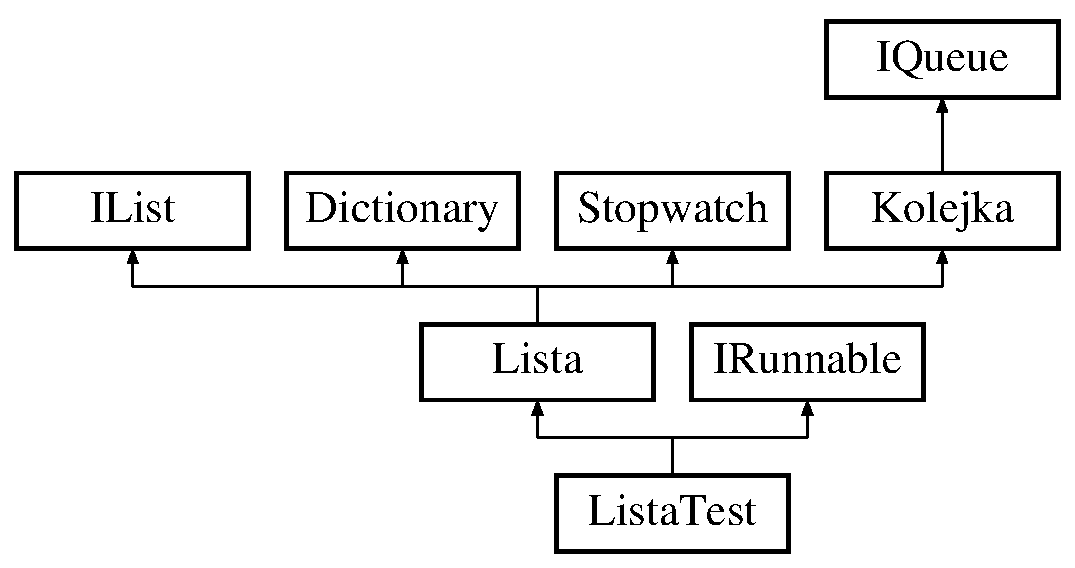
\includegraphics[height=4.000000cm]{class_lista_test}
\end{center}
\end{figure}
\subsection*{Public Member Functions}
\begin{DoxyCompactItemize}
\item 
void \hyperlink{class_lista_test_ad4f3d5d2eb57a4bd50e20664109e9d9b}{run} (int Amount\-Of\-Comp)
\end{DoxyCompactItemize}


\subsection{Member Function Documentation}
\hypertarget{class_lista_test_ad4f3d5d2eb57a4bd50e20664109e9d9b}{\index{Lista\-Test@{Lista\-Test}!run@{run}}
\index{run@{run}!ListaTest@{Lista\-Test}}
\subsubsection[{run}]{\setlength{\rightskip}{0pt plus 5cm}void Lista\-Test\-::run (
\begin{DoxyParamCaption}
\item[{int}]{Amount\-Of\-Comp}
\end{DoxyParamCaption}
)\hspace{0.3cm}{\ttfamily [virtual]}}}\label{class_lista_test_ad4f3d5d2eb57a4bd50e20664109e9d9b}
funkcja testujaca przeszukiwanie listy 
\begin{DoxyParams}{Parameters}
{\em Amount\-Of\-Comp} & \\
\hline
\end{DoxyParams}


Implements \hyperlink{class_i_runnable}{I\-Runnable}.



The documentation for this class was generated from the following files\-:\begin{DoxyCompactItemize}
\item 
Lista\-Test.\-h\item 
Lista\-Test.\-cpp\end{DoxyCompactItemize}

\hypertarget{class_sorting_alg}{\section{Sorting\-Alg Class Reference}
\label{class_sorting_alg}\index{Sorting\-Alg@{Sorting\-Alg}}
}
\subsection*{Public Member Functions}
\begin{DoxyCompactItemize}
\item 
void \hyperlink{class_sorting_alg_a78d0945155e34b6479bcda9fc809cd55}{bubble} (int $\ast$tab, int n)
\end{DoxyCompactItemize}


\subsection{Member Function Documentation}
\hypertarget{class_sorting_alg_a78d0945155e34b6479bcda9fc809cd55}{\index{Sorting\-Alg@{Sorting\-Alg}!bubble@{bubble}}
\index{bubble@{bubble}!SortingAlg@{Sorting\-Alg}}
\subsubsection[{bubble}]{\setlength{\rightskip}{0pt plus 5cm}void Sorting\-Alg\-::bubble (
\begin{DoxyParamCaption}
\item[{int $\ast$}]{tab, }
\item[{int}]{n}
\end{DoxyParamCaption}
)}}\label{class_sorting_alg_a78d0945155e34b6479bcda9fc809cd55}
funkcja sortujaca wykorzystujaca sortowanie babelkowe 
\begin{DoxyParams}{Parameters}
{\em tab} & -\/ wskaznik do tablicy, ktorej elementy maja zostac posortowane \\
\hline
{\em n} & -\/ rozmiar tablicy \\
\hline
\end{DoxyParams}


The documentation for this class was generated from the following files\-:\begin{DoxyCompactItemize}
\item 
Sorting\-Alg.\-h\item 
Sorting\-Alg.\-cpp\end{DoxyCompactItemize}

\hypertarget{class_stopwatch}{\section{Stopwatch Class Reference}
\label{class_stopwatch}\index{Stopwatch@{Stopwatch}}
}
Inheritance diagram for Stopwatch\-:\begin{figure}[H]
\begin{center}
\leavevmode
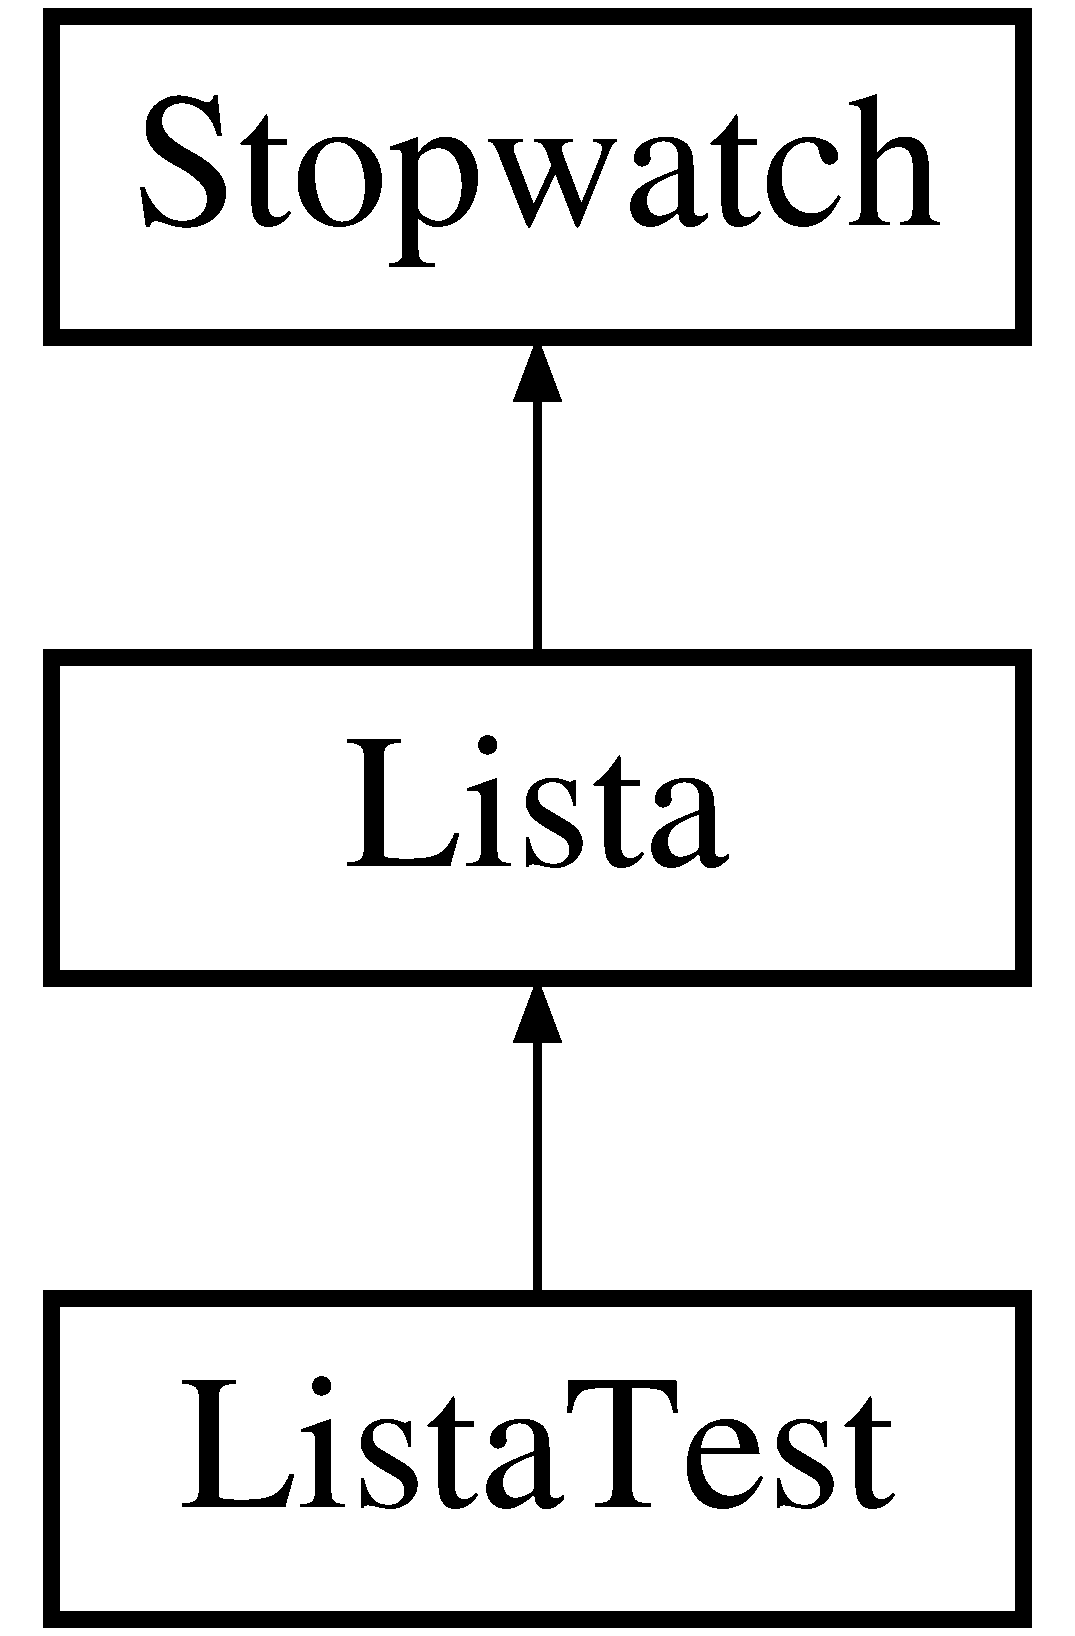
\includegraphics[height=3.000000cm]{class_stopwatch}
\end{center}
\end{figure}
\subsection*{Public Member Functions}
\begin{DoxyCompactItemize}
\item 
\hyperlink{class_stopwatch_a628b5ebeed5df065dd847e68fb6336cf}{Stopwatch} ()
\item 
virtual \hyperlink{class_stopwatch_a534c433482f8fe8144c91c0fe37aac20}{$\sim$\-Stopwatch} ()
\item 
double \hyperlink{class_stopwatch_a94fa586bb50e66c8713567b3c3d49363}{get\-Run\-Time} ()
\item 
void \hyperlink{class_stopwatch_affb208f2087bb95be62232adf117ebea}{set\-Run\-Time} ()
\item 
void \hyperlink{class_stopwatch_aac06497444e903787e2e8ba1db655485}{send\-To\-File} (int number)
\item 
clock\-\_\-t \hyperlink{class_stopwatch_ae85311604f23b21dabd7278f98f85982}{get\-Start} ()
\item 
void \hyperlink{class_stopwatch_a96e09b8ef0f10f11f1dc706e0f028464}{set\-Start} ()
\item 
clock\-\_\-t \hyperlink{class_stopwatch_a056cb3dedc2fbb7c415e5960d84d60d8}{get\-Stop} ()
\item 
void \hyperlink{class_stopwatch_a1d7ba5e1ccd82dedc13ebaf9a7c444ab}{set\-Stop} ()
\end{DoxyCompactItemize}


\subsection{Constructor \& Destructor Documentation}
\hypertarget{class_stopwatch_a628b5ebeed5df065dd847e68fb6336cf}{\index{Stopwatch@{Stopwatch}!Stopwatch@{Stopwatch}}
\index{Stopwatch@{Stopwatch}!Stopwatch@{Stopwatch}}
\subsubsection[{Stopwatch}]{\setlength{\rightskip}{0pt plus 5cm}Stopwatch\-::\-Stopwatch (
\begin{DoxyParamCaption}
{}
\end{DoxyParamCaption}
)}}\label{class_stopwatch_a628b5ebeed5df065dd847e68fb6336cf}
konstruktor \hypertarget{class_stopwatch_a534c433482f8fe8144c91c0fe37aac20}{\index{Stopwatch@{Stopwatch}!$\sim$\-Stopwatch@{$\sim$\-Stopwatch}}
\index{$\sim$\-Stopwatch@{$\sim$\-Stopwatch}!Stopwatch@{Stopwatch}}
\subsubsection[{$\sim$\-Stopwatch}]{\setlength{\rightskip}{0pt plus 5cm}Stopwatch\-::$\sim$\-Stopwatch (
\begin{DoxyParamCaption}
{}
\end{DoxyParamCaption}
)\hspace{0.3cm}{\ttfamily [virtual]}}}\label{class_stopwatch_a534c433482f8fe8144c91c0fe37aac20}
destruktor 

\subsection{Member Function Documentation}
\hypertarget{class_stopwatch_a94fa586bb50e66c8713567b3c3d49363}{\index{Stopwatch@{Stopwatch}!get\-Run\-Time@{get\-Run\-Time}}
\index{get\-Run\-Time@{get\-Run\-Time}!Stopwatch@{Stopwatch}}
\subsubsection[{get\-Run\-Time}]{\setlength{\rightskip}{0pt plus 5cm}double Stopwatch\-::get\-Run\-Time (
\begin{DoxyParamCaption}
{}
\end{DoxyParamCaption}
)}}\label{class_stopwatch_a94fa586bb50e66c8713567b3c3d49363}
funkcja zwracajaca czas wykonania \begin{DoxyReturn}{Returns}
Run\-Time\-\_\- 
\end{DoxyReturn}
\hypertarget{class_stopwatch_ae85311604f23b21dabd7278f98f85982}{\index{Stopwatch@{Stopwatch}!get\-Start@{get\-Start}}
\index{get\-Start@{get\-Start}!Stopwatch@{Stopwatch}}
\subsubsection[{get\-Start}]{\setlength{\rightskip}{0pt plus 5cm}clock\-\_\-t Stopwatch\-::get\-Start (
\begin{DoxyParamCaption}
{}
\end{DoxyParamCaption}
)}}\label{class_stopwatch_ae85311604f23b21dabd7278f98f85982}
funkcja zwracajaca czas rozpoczecia pomiaru \begin{DoxyReturn}{Returns}
start\-\_\- 
\end{DoxyReturn}
\hypertarget{class_stopwatch_a056cb3dedc2fbb7c415e5960d84d60d8}{\index{Stopwatch@{Stopwatch}!get\-Stop@{get\-Stop}}
\index{get\-Stop@{get\-Stop}!Stopwatch@{Stopwatch}}
\subsubsection[{get\-Stop}]{\setlength{\rightskip}{0pt plus 5cm}clock\-\_\-t Stopwatch\-::get\-Stop (
\begin{DoxyParamCaption}
{}
\end{DoxyParamCaption}
)}}\label{class_stopwatch_a056cb3dedc2fbb7c415e5960d84d60d8}
funkcja zwracajaca czas zakonczenia pomiaru \begin{DoxyReturn}{Returns}
stop\-\_\- 
\end{DoxyReturn}
\hypertarget{class_stopwatch_aac06497444e903787e2e8ba1db655485}{\index{Stopwatch@{Stopwatch}!send\-To\-File@{send\-To\-File}}
\index{send\-To\-File@{send\-To\-File}!Stopwatch@{Stopwatch}}
\subsubsection[{send\-To\-File}]{\setlength{\rightskip}{0pt plus 5cm}void Stopwatch\-::send\-To\-File (
\begin{DoxyParamCaption}
\item[{int}]{number}
\end{DoxyParamCaption}
)}}\label{class_stopwatch_aac06497444e903787e2e8ba1db655485}
funkcja zapisujaca pomiar w pliku 
\begin{DoxyParams}{Parameters}
{\em number} & -\/ liczba elementow dla ktorych dzialal algorytm \\
\hline
\end{DoxyParams}
\hypertarget{class_stopwatch_affb208f2087bb95be62232adf117ebea}{\index{Stopwatch@{Stopwatch}!set\-Run\-Time@{set\-Run\-Time}}
\index{set\-Run\-Time@{set\-Run\-Time}!Stopwatch@{Stopwatch}}
\subsubsection[{set\-Run\-Time}]{\setlength{\rightskip}{0pt plus 5cm}void Stopwatch\-::set\-Run\-Time (
\begin{DoxyParamCaption}
{}
\end{DoxyParamCaption}
)}}\label{class_stopwatch_affb208f2087bb95be62232adf117ebea}
funkcja obliczajaca czas wykonania algorytmu \hypertarget{class_stopwatch_a96e09b8ef0f10f11f1dc706e0f028464}{\index{Stopwatch@{Stopwatch}!set\-Start@{set\-Start}}
\index{set\-Start@{set\-Start}!Stopwatch@{Stopwatch}}
\subsubsection[{set\-Start}]{\setlength{\rightskip}{0pt plus 5cm}void Stopwatch\-::set\-Start (
\begin{DoxyParamCaption}
{}
\end{DoxyParamCaption}
)}}\label{class_stopwatch_a96e09b8ef0f10f11f1dc706e0f028464}
funkcja wlaczajaca stoper \hypertarget{class_stopwatch_a1d7ba5e1ccd82dedc13ebaf9a7c444ab}{\index{Stopwatch@{Stopwatch}!set\-Stop@{set\-Stop}}
\index{set\-Stop@{set\-Stop}!Stopwatch@{Stopwatch}}
\subsubsection[{set\-Stop}]{\setlength{\rightskip}{0pt plus 5cm}void Stopwatch\-::set\-Stop (
\begin{DoxyParamCaption}
{}
\end{DoxyParamCaption}
)}}\label{class_stopwatch_a1d7ba5e1ccd82dedc13ebaf9a7c444ab}
funkcja wylaczajaca stoper 

The documentation for this class was generated from the following files\-:\begin{DoxyCompactItemize}
\item 
Stopwatch.\-h\item 
Stopwatch.\-cpp\end{DoxyCompactItemize}

\hypertarget{class_stos}{\section{Stos Class Reference}
\label{class_stos}\index{Stos@{Stos}}
}
Inheritance diagram for Stos\-:\begin{figure}[H]
\begin{center}
\leavevmode
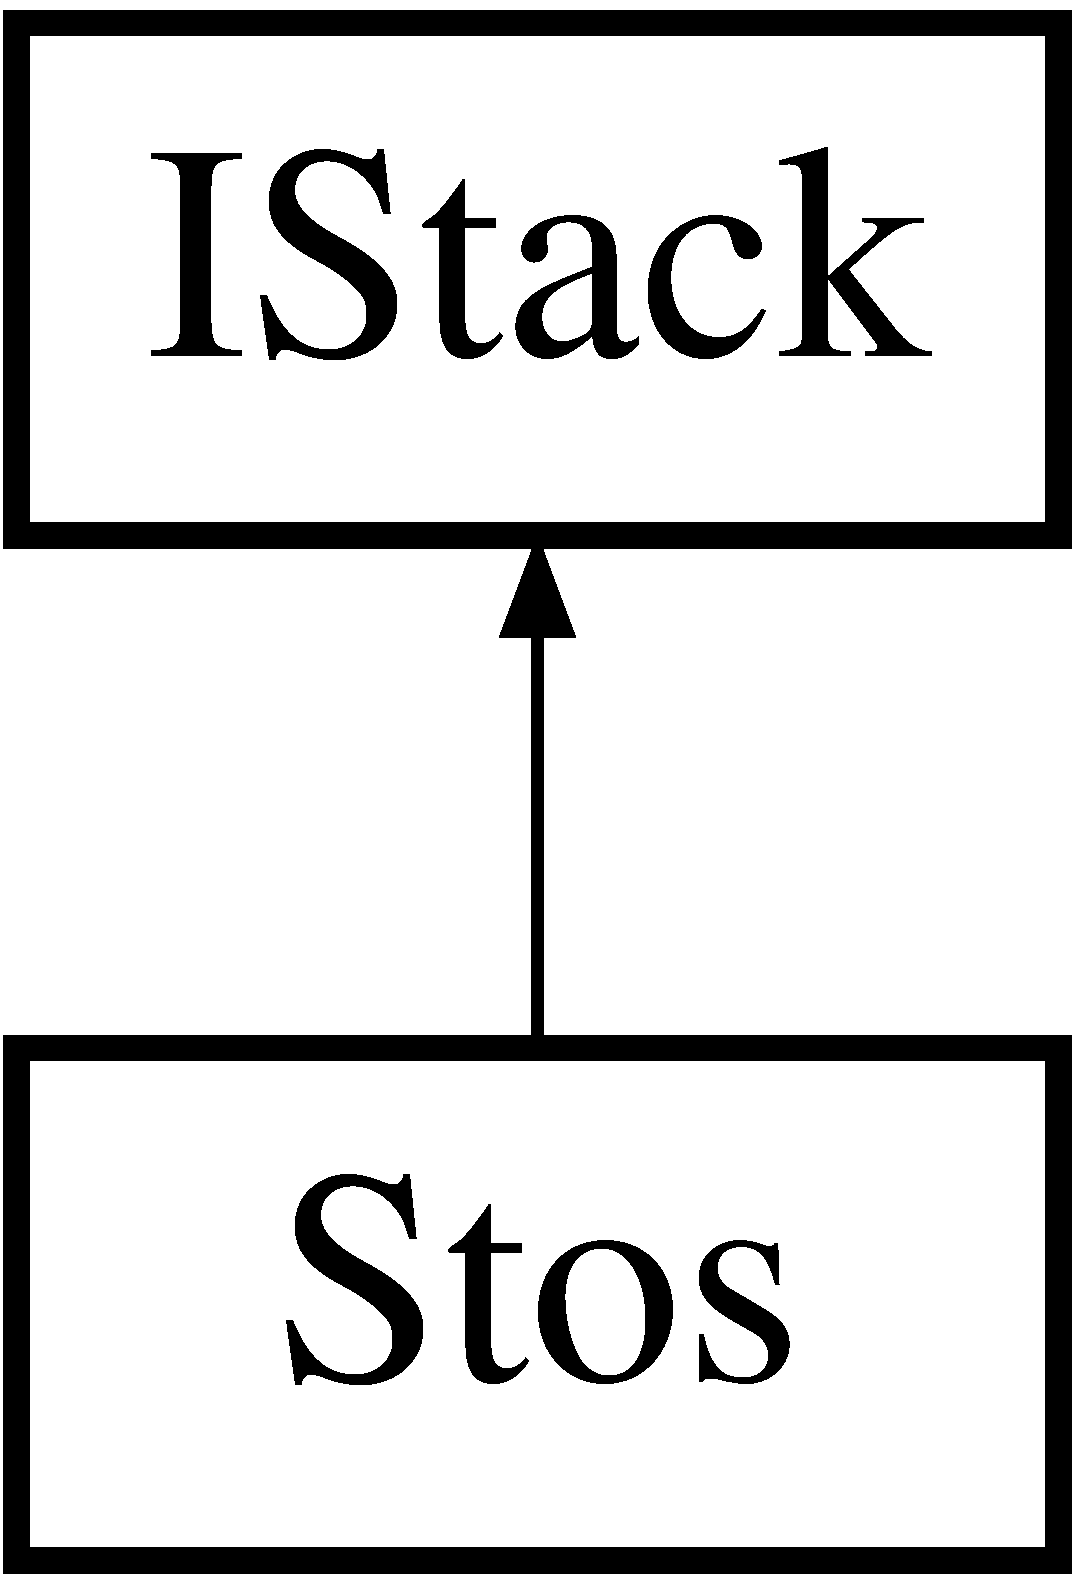
\includegraphics[height=2.000000cm]{class_stos}
\end{center}
\end{figure}
\subsection*{Public Member Functions}
\begin{DoxyCompactItemize}
\item 
\hyperlink{class_stos_a1de3b50386d5dfb56ddece17d0ea2389}{Stos} ()
\item 
virtual \hyperlink{class_stos_af9a198e2540e18adcc0b5259105fd78e}{$\sim$\-Stos} ()
\item 
void \hyperlink{class_stos_a8e592e006bfeb1fc678a9863a3156cf3}{push} (int a)
\item 
int \hyperlink{class_stos_a0aa50af4e55b9ceba61b44e33ef8dce2}{get\-Size} ()
\item 
int \hyperlink{class_stos_a83d252074388f18d49a950b6d312cc71}{top} ()
\item 
void \hyperlink{class_stos_a88b0da41b49ef4d4b63cfd4924665683}{pop} ()
\item 
bool \hyperlink{class_stos_a328eb30ceb157893dead1a9fe17597b7}{is\-Empty} ()
\item 
void \hyperlink{class_stos_a0afce6a79befd5b9b5663d75e0b92e7f}{enlarge\-\_\-x2} ()
\end{DoxyCompactItemize}


\subsection{Constructor \& Destructor Documentation}
\hypertarget{class_stos_a1de3b50386d5dfb56ddece17d0ea2389}{\index{Stos@{Stos}!Stos@{Stos}}
\index{Stos@{Stos}!Stos@{Stos}}
\subsubsection[{Stos}]{\setlength{\rightskip}{0pt plus 5cm}Stos\-::\-Stos (
\begin{DoxyParamCaption}
{}
\end{DoxyParamCaption}
)}}\label{class_stos_a1de3b50386d5dfb56ddece17d0ea2389}
konstruktor stack\-\_\- -\/ wskaznik do tablicy dynamicznej ze stosem; size\-\_\- -\/ poczatkowy rozmiar stosu; top\-\_\- -\/ nr indeksu elementu na wierzchu; count -\/ aktualna liczba elementow na stosie; \hypertarget{class_stos_af9a198e2540e18adcc0b5259105fd78e}{\index{Stos@{Stos}!$\sim$\-Stos@{$\sim$\-Stos}}
\index{$\sim$\-Stos@{$\sim$\-Stos}!Stos@{Stos}}
\subsubsection[{$\sim$\-Stos}]{\setlength{\rightskip}{0pt plus 5cm}Stos\-::$\sim$\-Stos (
\begin{DoxyParamCaption}
{}
\end{DoxyParamCaption}
)\hspace{0.3cm}{\ttfamily [virtual]}}}\label{class_stos_af9a198e2540e18adcc0b5259105fd78e}
destruktor 

\subsection{Member Function Documentation}
\hypertarget{class_stos_a0afce6a79befd5b9b5663d75e0b92e7f}{\index{Stos@{Stos}!enlarge\-\_\-x2@{enlarge\-\_\-x2}}
\index{enlarge\-\_\-x2@{enlarge\-\_\-x2}!Stos@{Stos}}
\subsubsection[{enlarge\-\_\-x2}]{\setlength{\rightskip}{0pt plus 5cm}void Stos\-::enlarge\-\_\-x2 (
\begin{DoxyParamCaption}
{}
\end{DoxyParamCaption}
)}}\label{class_stos_a0afce6a79befd5b9b5663d75e0b92e7f}
funkcja zwiekszajaca rozmiar stosu dwukrotnie \hypertarget{class_stos_a0aa50af4e55b9ceba61b44e33ef8dce2}{\index{Stos@{Stos}!get\-Size@{get\-Size}}
\index{get\-Size@{get\-Size}!Stos@{Stos}}
\subsubsection[{get\-Size}]{\setlength{\rightskip}{0pt plus 5cm}int Stos\-::get\-Size (
\begin{DoxyParamCaption}
{}
\end{DoxyParamCaption}
)}}\label{class_stos_a0aa50af4e55b9ceba61b44e33ef8dce2}
funkcja zwracajaca rozmiar stosu \begin{DoxyReturn}{Returns}
size\-\_\- 
\end{DoxyReturn}
\hypertarget{class_stos_a328eb30ceb157893dead1a9fe17597b7}{\index{Stos@{Stos}!is\-Empty@{is\-Empty}}
\index{is\-Empty@{is\-Empty}!Stos@{Stos}}
\subsubsection[{is\-Empty}]{\setlength{\rightskip}{0pt plus 5cm}bool Stos\-::is\-Empty (
\begin{DoxyParamCaption}
{}
\end{DoxyParamCaption}
)}}\label{class_stos_a328eb30ceb157893dead1a9fe17597b7}
funkcja sprawdzajaca, czy stos jest pusty \begin{DoxyReturn}{Returns}
-\/ zwraca 1 gdy pusty, 0 gdy niepusty 
\end{DoxyReturn}
\hypertarget{class_stos_a88b0da41b49ef4d4b63cfd4924665683}{\index{Stos@{Stos}!pop@{pop}}
\index{pop@{pop}!Stos@{Stos}}
\subsubsection[{pop}]{\setlength{\rightskip}{0pt plus 5cm}void Stos\-::pop (
\begin{DoxyParamCaption}
{}
\end{DoxyParamCaption}
)}}\label{class_stos_a88b0da41b49ef4d4b63cfd4924665683}
funkcja zdejmujaca ze stosu element z wierzchu \hypertarget{class_stos_a8e592e006bfeb1fc678a9863a3156cf3}{\index{Stos@{Stos}!push@{push}}
\index{push@{push}!Stos@{Stos}}
\subsubsection[{push}]{\setlength{\rightskip}{0pt plus 5cm}void Stos\-::push (
\begin{DoxyParamCaption}
\item[{int}]{a}
\end{DoxyParamCaption}
)}}\label{class_stos_a8e592e006bfeb1fc678a9863a3156cf3}
funkcja dokladajaca element na wierzch stosu 
\begin{DoxyParams}{Parameters}
{\em a} & -\/ element, ktory ma byc dodany \\
\hline
\end{DoxyParams}
\hypertarget{class_stos_a83d252074388f18d49a950b6d312cc71}{\index{Stos@{Stos}!top@{top}}
\index{top@{top}!Stos@{Stos}}
\subsubsection[{top}]{\setlength{\rightskip}{0pt plus 5cm}int Stos\-::top (
\begin{DoxyParamCaption}
{}
\end{DoxyParamCaption}
)}}\label{class_stos_a83d252074388f18d49a950b6d312cc71}
funkcja zwracajaca wartosc elementu na wierzchu stosu \begin{DoxyReturn}{Returns}
stack\-\_\-\mbox{[}top\-\_\-\mbox{]} 
\end{DoxyReturn}


The documentation for this class was generated from the following files\-:\begin{DoxyCompactItemize}
\item 
Stos.\-h\item 
Stos.\-cpp\end{DoxyCompactItemize}

%--- End generated contents ---

% Index
\newpage
\phantomsection
\addcontentsline{toc}{chapter}{Index}
\printindex

\end{document}
